\renewcommand{\baselinestretch}{1.2}
\usefonttheme[onlymath]{serif}
\title[Market Power and Contagion]{Market Power and Contagion in Interbank Networks}
\subtitle{An Agent-Based Model of Systemic Risk}

\author{Héctor~Castillo~Andreu}

\institute{
   Departament d'Economia\\
  Universitat Jaume~I
}

\date{19 June 2026}

\subject{Analysis through Agent-Based Models (ABM)}

\pgfdeclareimage[height=.4cm]{university-logo}{img/uji}
\logo{\pgfuseimage{university-logo}}

\AtBeginSection[]
{
  \begin{frame}<beamer>
    \frametitle{Outline}
    \tableofcontents[currentsection]
  \end{frame}
}

\newcommand{\photo}[2][.85]{%
  \begin{center}
    \includegraphics[width=#1\linewidth]{img/#2}
  \end{center}
}

\newcounter{slidenumber}
\newcommand{\frametitlecont}[1]{%
  \frametitle{#1 (\roman{slidenumber})}%
}

%======================================================================
\begin{document}

\setbeamertemplate{footline}{%
  \leavevmode%
  \hbox{%
  \begin{beamercolorbox}[wd=.5\paperwidth,ht=2.5ex,dp=1.125ex,leftskip=.3cm plus1fil,rightskip=.3cm]{author in head/foot}%
    \usebeamerfont{author in head/foot}\insertshortauthor
  \end{beamercolorbox}%
  \begin{beamercolorbox}[wd=.5\paperwidth,ht=2.5ex,dp=1.125ex,leftskip=.3cm,rightskip=.3cm plus1fil]{title in head/foot}%
    \usebeamerfont{title in head/foot}\insertframenumber\,/\,\inserttotalframenumber\ -- \insertshorttitle
  \end{beamercolorbox}}%
  \vskip0pt%
}

\begin{frame}
  \titlepage
\end{frame}

\begin{frame}<handout>[t,allowframebreaks]
  \frametitle{Outline}
  \tableofcontents
\end{frame}

%======================================================================
\section{Abstract}\label{sec:1}
%======================================================================

\begin{frame}{Abstract: ABM, Interbank Market, and Contagion}
  \begin{itemize}
    \item We use \textbf{Agent-Based Models} to study systemic risk in interbank credit networks.
    \item The dynamics are driven by two key parameters: the \textbf{probability of attachment} $p$ Erd\H{o}s--R\'enyi graphs as interbank connections generator (exogenous) and the \textbf{interest rate} $r$ (endogenous).
    \item As $p$ increases, the network becomes more connected, forming a giant component. Interest rates decline due to greater competition and reduced market power.
    \item However, higher connectivity also raises the probability of borrower bankruptcy. Excessively low interest rates, maintained for too long, can be \textbf{detrimental to the stability of the system}.
  \end{itemize}
\end{frame}

%======================================================================
\section{Risk and Connectivity}\label{sec:2}
%======================================================================

\begin{frame}{The 2008 Crisis: Background}
  \begin{itemize}
    \item A prolonged period of low interest rates encouraged excessive risk-taking and increased bank leverage.
    \item Standard competitive equilibrium models failed to capture the complex interactions that amplify crises.
    \item The interbank market became a \textbf{contagion vector}: failure of one bank triggered a domino effect through interlocking exposures, revealing how interconnectedness can magnify systemic fragility.
  \end{itemize}
\end{frame}

\begin{frame}{The Risk-Sharing Trade-off}
  Two opposing effects of network connectivity:
  \begin{itemize}
    \item \textbf{Benefit:} Increasing connectivity allows \textbf{risk sharing}---banks diversify exposure across more counterparties, lowering interest rates.
    \item \textbf{Cost:} Excessive connectivity increases \textbf{systemic risk}---default propagates through the network, and lenders serving a larger number of clients face higher bankruptcy exposure.
    \item Evidence: a \textbf{non-monotonic relationship} exists---low connectivity stabilizes by diluting shocks, but high connectivity facilitates cascading failures. Taken together, these effects imply that excessively low interest rates increase both bankruptcies and contagion.
  \end{itemize}
\end{frame}

% \begin{frame}{Empirical Evidence}
%   \begin{itemize}
%     \item Allen \& Gale (2000), Thurner et al. (2003), Iori et al. (2006): modeling credit systems as random graphs shows that bankruptcy avalanche probability \textbf{decreases} with connectivity.
%     \item Lorenz \& Battiston (2008) show that with \textbf{financial acceleration} (trend reinforcement in fragility), the probability of default does \textbf{not} decrease monotonically with connectivity.
%     \item Iori et al. (2006) identify \textbf{agent heterogeneity} as the root cause of bankruptcy avalanches.
%     %\item Financial crises are characterized by the \textbf{procyclicality of leverage} across institutions.
%     %\item Reserve requirements dampen cascades but \textbf{limit growth} by reducing firm investment.
%   \end{itemize}
% \end{frame}

\begin{frame}{Failure Channels in Financial Crises}
  In literature, three primary propagation mechanisms of systemic failure are identified:
  \begin{enumerate}
    \item \textbf{Bank runs:} self-fulfilling panics where depositors withdraw mass funds simultaneously.
    \item \textbf{Asset price contagion:} fire-sale spirals that depreciate assets across the system.
    \item \textbf{Interlocking exposures:} direct linkages through the interbank market---default of one bank triggers defaults in connected banks.
  \end{enumerate}
\end{frame}

\begin{frame}{Failure Channels in the Model}
  In this model, we consider the three failure channels:
  \begin{itemize}
    \item \textbf{Rationing} (insufficient funding of borrower),
    \item \textbf{Contagion} (lender suffers losses from borrower default),
    \item \textbf{Repayment failure} (borrower cannot repay loan).
  \end{itemize}
  At low connectivity: rationing dominates; at high connectivity, repayment failure becomes the primary risk.
\end{frame}



%======================================================================
\section{Model Framework}\label{sec:3}
%======================================================================

\begin{frame}{Model Overview}
  \begin{itemize}
    \item ABM with $N$ banks in a sequential economy $t = \{0, 1, \dots, T\}$.
    \item Banks connected through an \textbf{Erd\H{o}s--R\'enyi} random graph $G(N, p)$: each edge exists with exogenous probability $p$ (probability of attachment).
    \item The \textbf{interest rate} $r$ is the key endogenous variable determining loan relationships between borrowers and lenders.
    \item Goal: analyze how \textbf{connectivity} ($p$) and \textbf{market power} ($\psi$) affect system stability through the endogenous adjustment of $r$.
  \end{itemize}
\end{frame}

\begin{frame}{Balance Sheet}
  \begin{block}{Accounting Identity}
    \centering
    $L^t_i + C^t_i + R^t_i = D^t_i + E^t_i$
  \end{block}
  \begin{itemize}
    \item \textbf{Assets:} Long-term assets ($L$), liquidity ($C$), reserves ($R$).
    \item \textbf{Liabilities:} Deposits ($D$), equity ($E$).
    \item Reserves set by regulation: $R = \hat{r} D$ with $\hat{r} = 0.02$.
  \end{itemize}
\end{frame}

\begin{frame}{Liquidity Shocks}
  Deposits are exogenously shocked each period:
  \begin{block}{}
    \centering
    $ D^t_i = D^{t-1}_i [\mu + \omega \cdot U(0,1)]$
  \end{block}
  \begin{itemize}
    \item $\mu=0.7$: expected growth rate.
    \item $\omega=0.35  $: shock magnitude.
    \item \textbf{Potential lenders:} banks with supply of $C$ (after rebalance).
    \item \textbf{Potential borrowers:} banks with demand of loan ($C < 0$).
  \end{itemize}
\end{frame}


\begin{frame}{Network Structure}
  \begin{itemize}
    \item Bilateral credit lines formed at the start of each period.
    \item Connectivity controlled by parameter $p$ in the Erd\H{o}s--R\'enyi graph.
    \item Each borrower is matched to \textbf{exactly one} lender per period.
    \item The \textbf{Giant Component Size (GCS)} measures network integration.
  \end{itemize}
\end{frame}

{\usebackgroundtemplate{%
  \vbox to 0pt{\vskip40pt\hbox{\hskip30pt
\includegraphics[width=0.9\paperwidth,height=0.85\paperheight,keepaspectratio]{with_directions.png}}\vss}%
}
\begin{frame}[t]
  \frametitle{Erd\H{o}s--R\'enyi Random Graph}
  \vspace{0.5cm}
  \begin{minipage}{0.85\textwidth}
    \vspace{3.5cm}
    \footnotesize
    Each of the $\binom{N}{2}$ edges is included independently with prob. $p$. For $N=20$ banks:
    \begin{itemize}
      \item $p = 0$: isolated banks, no interbank market.
      \item $p = 1/N = 0.05$: \textbf{phase transition}: giant component begins to emerge.
      \item $p > 0.105$: network is saturated ($>92\%$ of banks connected): \textbf{supercritical regime}.
    \end{itemize}
  \end{minipage}
\end{frame}
}



\begin{frame}{Network Structure}
The Erd\H{o}s--R\'enyi model does not attempt to replicate the entire interbank market; rather, it illustrates how connection density alters the probability and scale of contagion.
\end{frame}


%======================================================================
\section{Interest Rate and Market Power}\label{sec:4}
%======================================================================


\begin{frame}{Expected Profit}
  Banks are risk-neutral in perfect competition. Expected profit for lender $i$ from lending to borrower $j$:
  \begin{block}{}
    \centering
    $\mathbb{E}[\Pi_t^{i,j}] = \underbrace { p_t^j (r_t^{i,j} c_t^{i,j} - \overbrace {m \, c^{i,j}_t}^{\text{cost of loan}}) }_{\text{normally pays}}- \underbrace {(1 - p_t^j)(m \, c_t^{i,j})}_{\text{when fails}} $

    % $E[\Pi_{i,j}^t] = p_j^t (r_{i,j}^t - m) c_{i,j}^t - (1 - p_j^t) m \cdot c_{i,j}^t$
  \end{block}
  \begin{itemize}
    \item $m$: screening cost ($0.015$).
    \item $p_j^t$: probability of borrower survival.
    \item $r_{i,j}^t$: interest rate; $c_{i,j}^t$: lending capacity.
%    \item The interest rate is the key variable determining the profitability and risk of each loan relationship.
  \end{itemize}
\end{frame}

\begin{frame}{Interest Rate Derivation}
  Setting $E[\Pi] = 0$ (zero-profit condition): $r_{i,j}^t = \frac{m}{p_j^t}$. \\
  Introducing \textbf{market power} $\psi \in [0,1]$:
  \begin{block}{}
    \centering
    $ r_{i,j}^t = \frac{m}{p_j^t (1 - \psi)} $
  \end{block}
  \begin{itemize}
    \item $\psi = 0$: competitive rate.
    \item $\psi > 0$: monopolistic markup from information asymmetry.
    \item As connectivity $p$ increases, competition intensifies, market power $\psi$ declines, and the interest rate falls.
  \end{itemize}
\end{frame}

\begin{frame}{Endogenous Market Power}
  Market power evolves endogenously with bank size:
  \begin{block}{}
    \centering
    $ \psi_i^t = \frac{E_i^t}{E_i^{t,\max}} $
  \end{block}
  \begin{itemize}
    \item Larger banks (higher equity) exercise more market power.
    \item Borrower default probability:
    $p_{b,j}^t = E_j^t / E_j^{t,\max}$.
    \item Leverage: $\lambda_j^t = d_j^t / E_j^t$.
    \item As $p$ increases, the market becomes more competitive\ --- borrowers can choose among more lenders, reducing lenders' market power. However, this also allows lenders to serve more clients, increasing their exposure to borrower default.
  \end{itemize}
\end{frame}



%======================================================================
\section{Equity and Bankruptcy Dynamics}\label{sec:5}
%======================================================================

\begin{frame}{Equity Evolution}
   \begin{block}{}
    \centering
    $ E^t_i = E^{t-1}_i + \sum_{j} l^{t}_{i,j} r^{t}_{i,j} - \sum_{j \subseteq \theta^t_i} \left[ B^{t}_{i,j} - \tilde{L}^t_j \right] $
  \end{block} 
  \begin{itemize}
    \item \textbf{Bankruptcy:} bank exits if $E_i^t < 0$.
    \item \textbf{Fire sales:} last-resort option (blocked in this model to amplify contagion effects).
    \item Failed banks replaced by new entrants with small initial capital.
    \item Endogenous interest rates affect bank earnings; low rates compress margins but also reduce the cost of borrowing, generating opposing effects on stability.
  \end{itemize}
\end{frame}


\begin{frame}{Failure Channels}
  Three distinct causes of bank failure:
  \begin{enumerate}
    \item \textbf{Rationing:} borrower cannot secure sufficient funding.
    \item \textbf{Contagion:} lender suffers losses from borrower default (bad debt).
    \item \textbf{Repayment failure:} fully-funded borrower cannot repay loan or interest.
  \end{enumerate}
  \vspace{0.3cm}
  \textbf{Rationing dominates} at low connectivity (fewer lending opportunities). \textbf{Repayment failure dominates} at high connectivity, as lenders serve more clients and the probability of borrower bankruptcy rises with lower interest rates.
\end{frame}



%======================================================================
\section{Phase Transition}\label{sec:6}
%======================================================================

\begin{frame}[shrink=0.1]{Phase Transition}
  \begin{itemize}
    \item \textbf{Phase transition:} GCS jumps from $\sim 1$ to $\sim 46$ banks ($92\%$) as $p$ crosses the phase transition (really above $p_c=1/N$).
    \item \textbf{Low $p$:} rationing-dominated, high interest rates ($r \approx 3.0$), few loans granted.
    \item \textbf{High $p$:} repayment-failure-dominated, low interest rates ($r \approx 1.8$), saturated network.
    \item As the market becomes more competitive, lenders serve more clients, the probability of bankruptcy rises, and bad debt accumulates.
  \end{itemize}
\end{frame}

\begin{frame}[shrink=0.1]{Phase Transition}

  \vspace{0.05cm}

  \begin{columns}[T]
    \begin{column}{0.55\textwidth}
      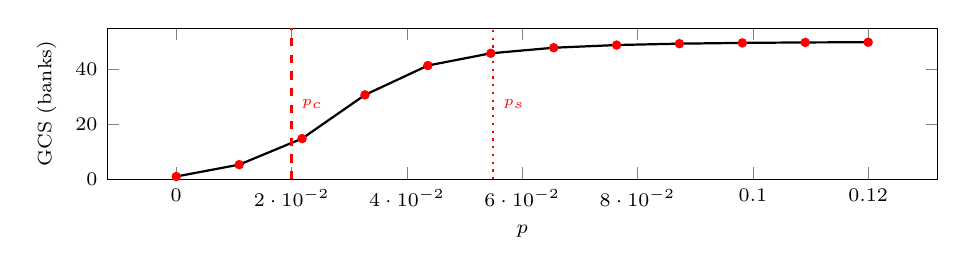
\begin{tikzpicture}
        \begin{axis}[
          width=\textwidth,
          height=3.5cm,
          xlabel={$p$},
          ylabel={GCS (banks)},
          ymin=0, ymax=55,
          font=\scriptsize,
        ]
        \addplot[red, only marks, mark=*, mark size=1.5pt] coordinates {
          (0.00001, 1.01)
          (0.01092, 5.33)
          (0.02183, 14.83)
          (0.03273, 30.72)
          (0.04364, 41.42)
          (0.05455, 45.87)
          (0.06546, 47.90)
          (0.07637, 48.88)
          (0.08727, 49.38)
          (0.09818, 49.66)
          (0.10909, 49.83)
          (0.12000, 49.90)
        };
        \addplot[black, thick] coordinates {
          (0.00001, 1.01)
          (0.01092, 5.33)
          (0.02183, 14.83)
          (0.03273, 30.72)
          (0.04364, 41.42)
          (0.05455, 45.87)
          (0.06546, 47.90)
          (0.07637, 48.88)
          (0.08727, 49.38)
          (0.09818, 49.66)
          (0.10909, 49.83)
          (0.12000, 49.90)
        };
        \draw[red, dashed, thick] (axis cs:0.02,0) -- (axis cs:0.02,55)
          node[pos=0.5, right, font=\tiny]{$p_c$};
        \draw[red, dotted, thick] (axis cs:0.055,0) -- (axis cs:0.055,55)
          node[pos=0.5, right, font=\tiny]{$p_s$};
        \end{axis}
      \end{tikzpicture}
      \vspace{0.1cm}      
      \tiny{        
        $\langle k \rangle = p(N-1)$
        }
      \vspace{0.2cm} \\
      \footnotesize          
      \textbf{Percolation threshold} $\langle k \rangle \approx 1$ (phase transition) for Erd\H{o}s--R\'enyi graph: \[
        p_c = \frac{1}{N} = \frac{1}{50} = 0.02
        \] \\
      \textbf{Supercritical region} $\langle k \rangle = 2.14$, observed at $p_s = 0.0436$. \\
        
    \end{column}
    \begin{column}{0.42\textwidth}
      \footnotesize
      \centering
      \begin{tabular}{rr}
        \toprule
        $p$ & GCS \\
        \midrule
        0.00001 & 1 \\
        0.011 & 5 \\
        \textbf{0.022} & \textbf{15} \\
        0.033 & 31 \\
        0.044 & 41 \\
        \textbf{0.055} & \textbf{46} \\
        0.065 & 48 \\
        0.087 & 49 \\
        $\geq 0.11$ & 50 \\
        \bottomrule
      \end{tabular}
    \end{column}
  \end{columns}
\end{frame}


% \begin{frame}{Connectivity and Systemic Risk}
%   \begin{itemize}
%     \item As $p$ increases, the interest rate drops from $30$ (upper bound) to $\sim 1.65$, reflecting reduced market power.
%     \item Bankruptcies remain stable at $\sim 7$--$7.5$, with the composition shifting from rationing to repayment failure.
%     \item Active loans saturate at $\sim 13$ ($26\%$ of banks), indicating that lenders can serve more clients.
%     \item Bad debt grows rapidly with connectivity (from $0$ to $\sim 1.3$), as more loans translate into higher default exposure.
%     \item Taken together, these results show that an interest rate that remains too low for too long can be \textbf{detrimental to the stability of the system}.
%   \end{itemize}
% \end{frame}

%======================================================================
\section{Results}\label{sec:7}
%======================================================================

% \begin{frame}{Bankruptcies exposed by the model}
%   \begin{columns}[T]
%     \begin{column}{0.9\textwidth}
%       \centering
%       \begin{tikzpicture}
%         \begin{axis}[
%           width=0.9\textwidth,
%           height=0.60\textheight,
%           ylabel={Rationing + Repayment},
%           ylabel style={font=\sffamily\tiny, yshift=-20pt},
%           ymin=0, ymax=8,
%           xmin=0, xmax=0.12,
%           xlabel={$p$},
%           xlabel style={font=\sffamily\tiny},
%           every axis x label/.style={at={(ticklabel* cs:0.5)}, yshift=-12pt, font=\sffamily\tiny},
%   every axis y label/.style={at={(axis description cs:-0.08,0.5)}, rotate=90, font=\sffamily\tiny},
%           xticklabel style={/pgf/number format/fixed, /pgf/number format/precision=2, font=\sffamily\tiny},
%           yticklabel style={font=\sffamily\tiny},
%           font=\sffamily\tiny,
%           tick style={black, line width=0.4pt},
%           major tick length=3pt,
%           axis line style={black},
%           ticklabel style={font=\sffamily\tiny},
%         ]
%           \addplot[only marks, mark=square*, red] coordinates {
%             (0.00001,6.7931)            (0.01100,6.1768)            (0.02200,6.4994)            (0.03300,6.5926)            (0.04400,6.6995)            (0.05500,6.7234)            (0.06500,6.7342)            (0.07600,6.7453)            (0.08700,6.8621)            (0.09800,6.7748)            (0.10900,6.7942)            (0.12000,6.8065)
%           };
%           \addplot[black, thick]coordinates {
%             (0.00001,6.7931)            (0.01100,6.1768)            (0.02200,6.4994)            (0.03300,6.5926)            (0.04400,6.6995)            (0.05500,6.7234)            (0.06500,6.7342)            (0.07600,6.7453)            (0.08700,6.8621)            (0.09800,6.7748)            (0.10900,6.7942)            (0.12000,6.8065)
%           };
%           \addplot[only marks, mark=o, red] coordinates {
%             (0.00001,0.00)            (0.01100,0.24)            (0.02200,0.45)            (0.03300,0.57)            (0.04400,0.67)            (0.05500,0.73)            (0.06500,0.78)            (0.07600,0.80)            (0.08700,0.84)            (0.09800,0.84)            (0.10900,0.84)            (0.12000,0.86)
%           };
%           \addplot[black, thick]coordinates {
%             (0.00001,0.00)            (0.01100,0.24)            (0.02200,0.45)            (0.03300,0.57)            (0.04400,0.67)            (0.05500,0.73)            (0.06500,0.78)            (0.07600,0.80)            (0.08700,0.84)            (0.09800,0.84)            (0.10900,0.84)            (0.12000,0.86)
%           };
%         \end{axis}
%         \begin{axis}[
%           width=0.9\textwidth,
%           height=0.60\textheight,
%           ylabel={Contagion},
%           ylabel style={font=\tiny},
%           ymin=0, ymax=0.4,
%           xmin=0, xmax=0.12,
%           axis y line*=right, axis x line=none,
%           ylabel near ticks,
%           yticklabel style={/pgf/number format/fixed, /pgf/number format/precision=2, font=\tiny},
%           font=\tiny,
%           ticklabel style={font=\tiny},
%         ]
%           \addplot[only marks, mark=*, red] coordinates {
%             (0.00001,0.0000)            (0.01100,0.0128)            (0.02200,0.0313)            (0.03300,0.0443)            (0.04400,0.0573)            (0.05500,0.0634)            (0.06500,0.0700)            (0.07600,0.0750)            (0.08700,0.0811)            (0.09800,0.0836)            (0.10900,0.0802)            (0.12000,0.0824)
%           };
%           \addplot[black, thick]coordinates {
%             (0.00001,0.0000)            (0.01100,0.0128)            (0.02200,0.0313)            (0.03300,0.0443)            (0.04400,0.0573)            (0.05500,0.0634)            (0.06500,0.0700)            (0.07600,0.0750)            (0.08700,0.0811)            (0.09800,0.0836)            (0.10900,0.0802)            (0.12000,0.0824)
%           };
%         \end{axis}
%         \end{tikzpicture}
%     \end{column}
%     \begin{column}{0.28\textwidth}
%       \centering
%       \tiny
%       \renewcommand{\arraystretch}{0.85}\setlength{\tabcolsep}{3pt}
%       \textcolor{red}{$\blacksquare$} Rationing
%       \textcolor{red}{$\bullet$} Contagion\par
%       \textcolor{red}{$\circ$} Repayment fail.\par
%       \vspace{0.15cm}
%       \begin{tabular}{lccc}
%         \toprule
%         $p$ & Rat. & Cont. & Fail. \\
%         \midrule
%         0.001 & 6.79 & 0.00 & 0.00 \\
%         0.011 & 6.18 & 0.01 & 0.24 \\
%         0.022 & 6.50 & 0.03 & 0.45 \\
%         0.033 & 6.59 & 0.04 & 0.57 \\
%         0.044 & 6.70 & 0.06 & 0.67 \\
%         \textbf{0.055} & \textbf{6.72} & \textbf{0.06} & \textbf{0.73} \\
%         0.065 & 6.73 & 0.07 & 0.78 \\
%         0.076 & 6.75 & 0.07 & 0.80 \\
%         0.087 & 6.86 & 0.08 & 0.84 \\
%         0.098 & 6.77 & 0.08 & 0.84 \\
%         0.109 & 6.79 & 0.08 & 0.84 \\
%         0.120 & 6.81 & 0.08 & 0.86 \\
%         \bottomrule
%       \end{tabular}


%     \end{column}

%   \end{columns}
%   \vspace{0.05cm}
% {\tiny
% \renewcommand{\baselinestretch}{0.85}\selectfont
% As $p$ increases, the channel of failure shifts from rationing (few lenders available) to repayment failure (low rates, more clients served). % This compositional change illustrates how excessive connectivity and low interest rates jointly increase systemic fragility.\\[-0.4em]


% \setlength{\tabcolsep}{3pt}
% \renewcommand{\arraystretch}{0.85}
% Initial conditions for each bank:
% \begin{tabular}{l|l}
%   \multicolumn{1}{c|}{\textbf{Assets}} & \multicolumn{1}{c}{\textbf{Liabilities}} \\ \midrule
%   $C^i_0= 5-0.18 = 4.82$ & $D^i_0= 9$\\
%   $L^i_0= 5$ & $E^i_0= 1$ \\
%   $R^i_0 = 0.18$ &
% \end{tabular}
% }
% \end{frame}


\begin{frame}{Bankruptcies}
 

  \begin{columns}[T]
    \begin{column}{0.75\textwidth}
      \begin{figure}
        \centering
        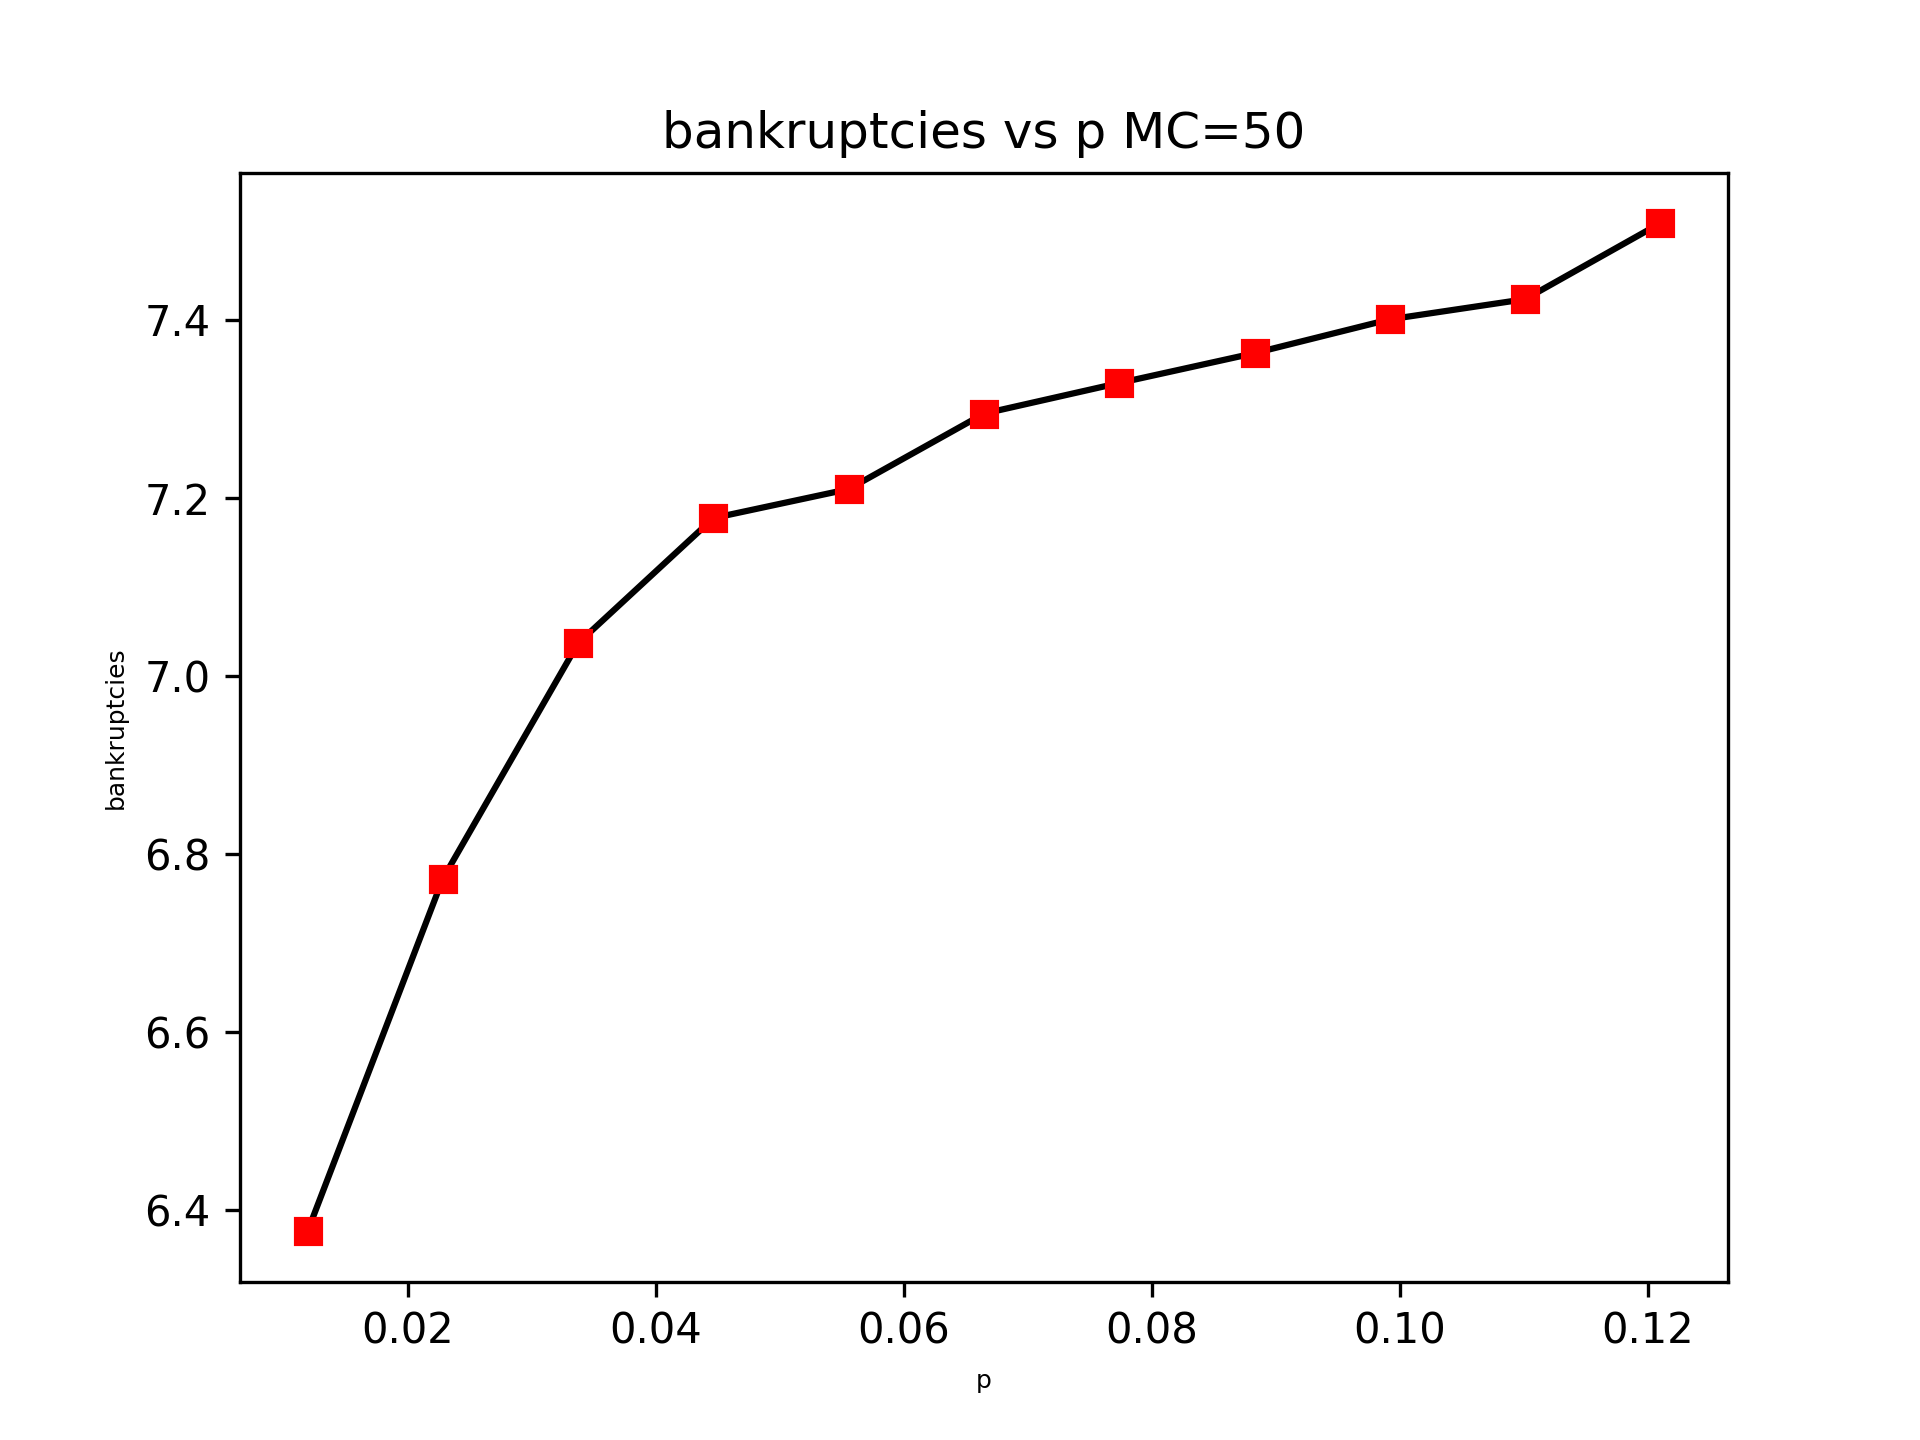
\includegraphics[width=\textwidth, trim=0 0 0 38, clip]{bankruptcies.png}
      \end{figure}
    \end{column}
    \begin{column}{0.23\textwidth}
      \centering
      \tiny\renewcommand{\arraystretch}{0.85}\setlength{\tabcolsep}{3pt}
      \begin{tabular}{lr}
        \toprule
        p & bankruptcies \\
        \midrule
        0.012 & 6.3762 \\
        0.023 & 6.7724 \\
        0.034 & 7.0369 \\
        0.045 & 7.1774 \\
        0.056 & 7.2100 \\
        0.066 & 7.2948 \\
        0.077 & 7.3292 \\
        0.088 & 7.3628 \\
        0.099 & 7.4007 \\
        0.110 & 7.4234 \\
        0.121 & 7.5088 \\
        \bottomrule
      \end{tabular}

      \vspace{0.5cm}
      Monte Carlo simulations with $\mathcal{MC} = 50$ runs. $N=50$ banks, $T=1000$ periods, and $p$ varying from 0 to 0.12 in increments of 0.01.

    \end{column}
  \end{columns}
  \tiny \setlength{\tabcolsep}{3pt}
  \renewcommand{\arraystretch}{0.85}
  Initial conditions for each bank:
  \begin{tabular}{l|l}
    \multicolumn{1}{c|}{\textbf{Assets}} & \multicolumn{1}{c}{\textbf{Liabilities}} \\ \midrule
    $C^i_0= 5-0.18 = 4.82$ & $D^i_0= 9$\\
    $L^i_0= 5$ & $E^i_0= 1$ \\
    $R^i_0 = 0.18$ &
  \end{tabular}
\end{frame}




\begin{frame}{Bankruptcies decomposition }
  \tiny As $p$ increases, the channel of failure shifts from rationing (few lenders available) to repayment failure (low rates, more clients served). % This compositional change illustrates how excessive connectivity and low interest rates jointly increase systemic fragility.\\[-0.4em]
Monte Carlo simulations with $\mathcal{MC} = 50$ runs. $N=50$ banks, $T=1000$ periods, and $p$ varying from 0 to 0.12 in increments of 0.01.
  \begin{columns}[T]
    \begin{column}{0.75\textwidth}
      \begin{figure}
        \centering
        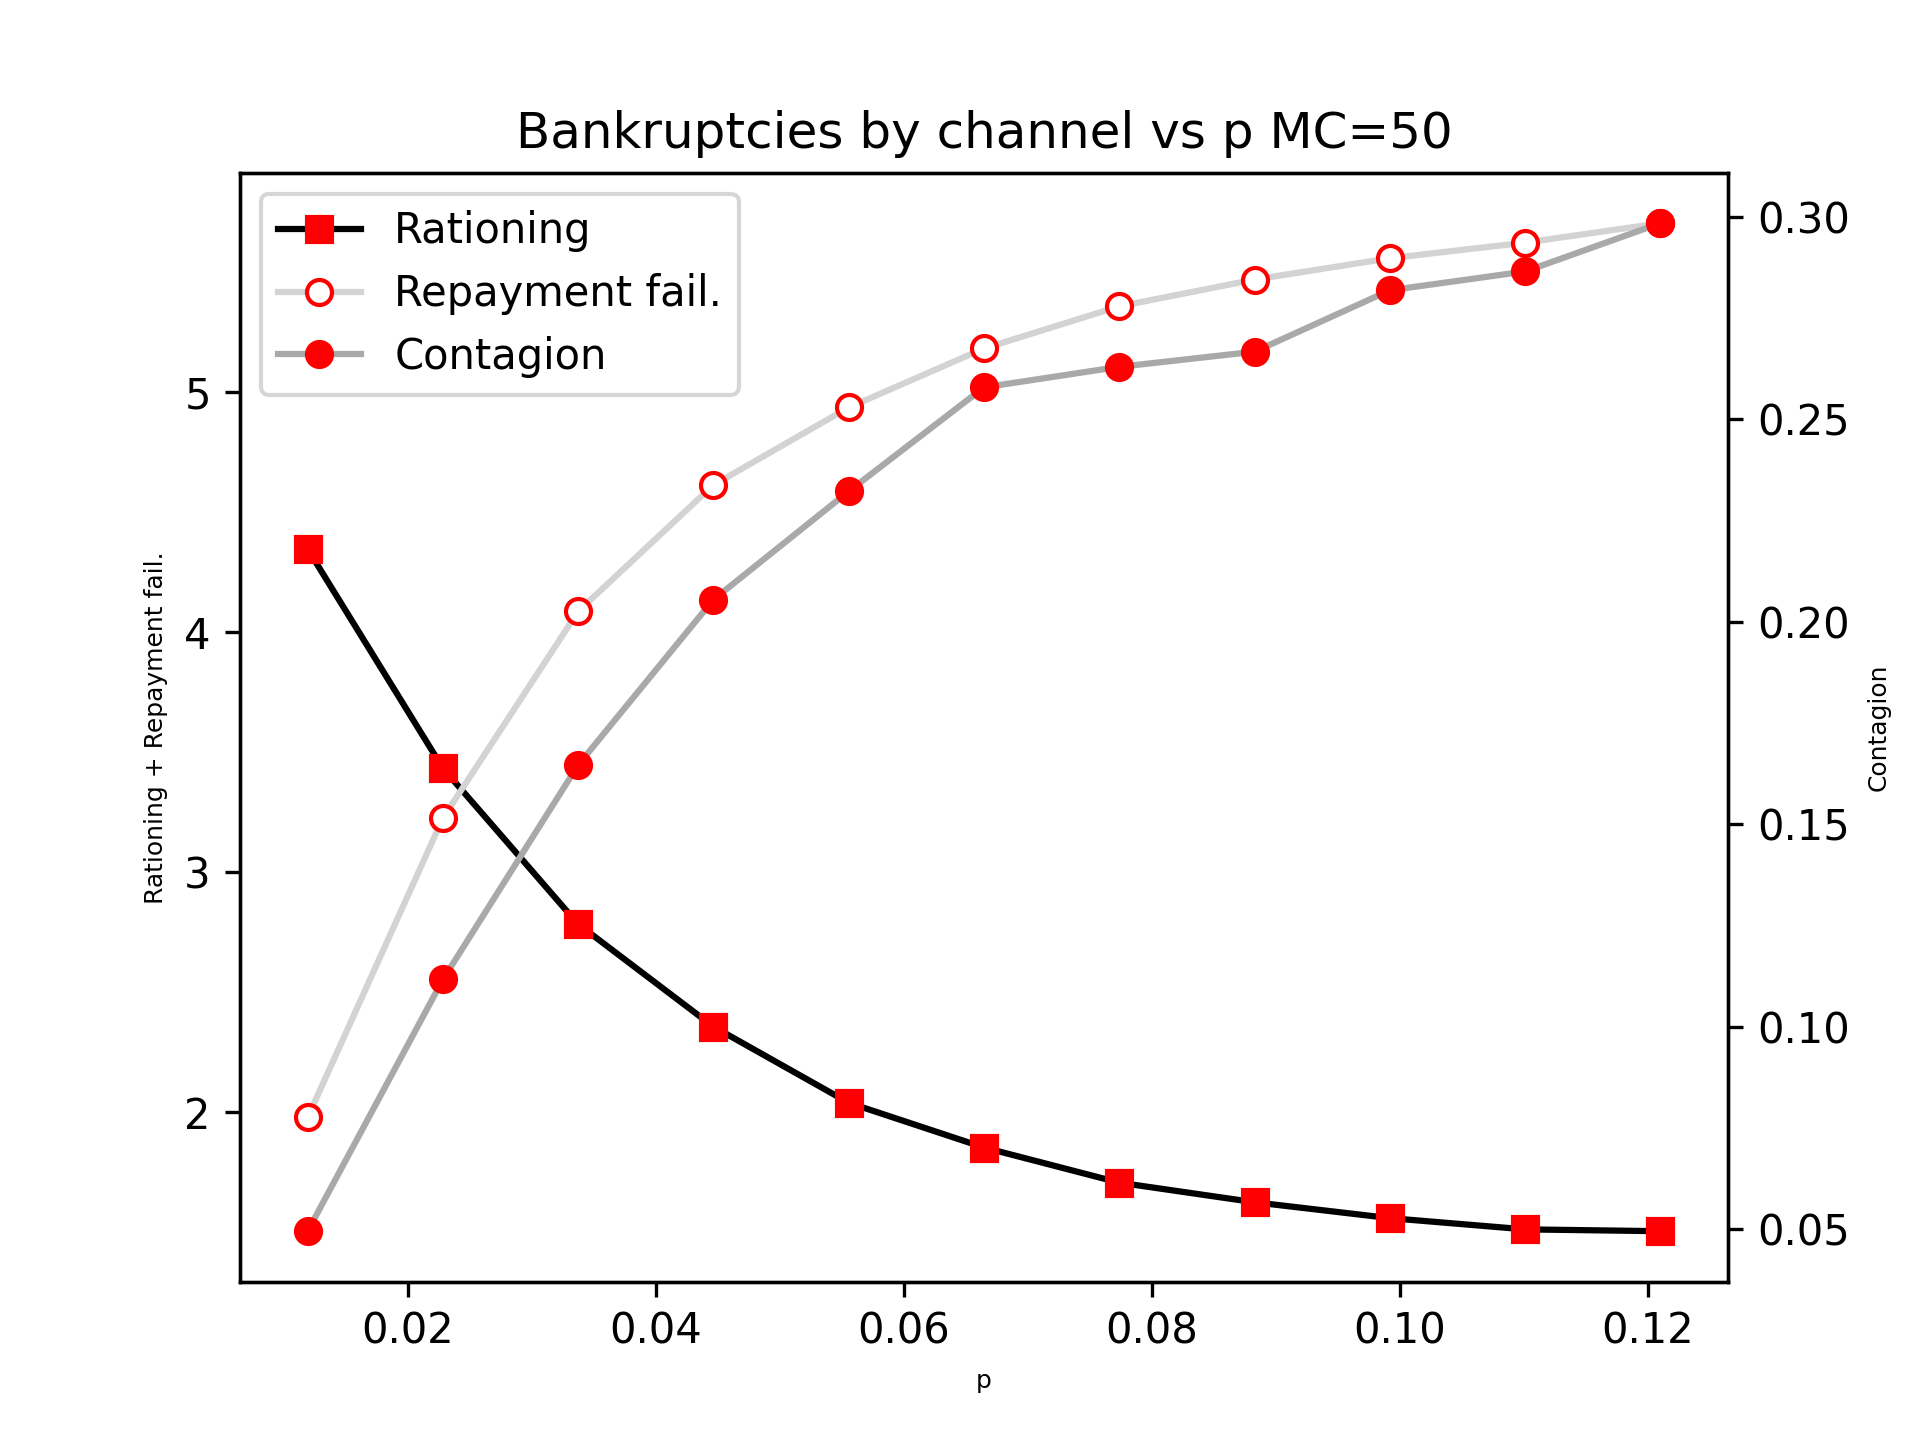
\includegraphics[width=\textwidth, trim=0 0 0 38, clip]{bankruptcies_all.png}
      \end{figure}
    \end{column}
    \begin{column}{0.23\textwidth}
      \renewcommand{\arraystretch}{0.85}\setlength{\tabcolsep}{3pt}
      \begin{tabular}{lrrr}
        \toprule
        $p$ & Rat. & Cont. & Fail. \\
        \midrule
        0.012 & 4.35 & 0.05 & 1.98 \\
        0.023 & 3.43 & 0.11 & 3.23 \\
        0.034 & 2.78 & 0.16 & 4.09 \\
        0.045 & 2.36 & 0.21 & 4.61 \\
        0.056 & 2.04 & 0.23 & 4.94 \\
        0.066 & 1.85 & 0.26 & 5.18 \\
        0.077 & 1.71 & 0.26 & 5.36 \\
        0.088 & 1.63 & 0.27 & 5.47 \\
        0.099 & 1.56 & 0.28 & 5.56 \\
        0.110 & 1.51 & 0.29 & 5.62 \\
        0.121 & 1.51 & 0.30 & 5.71 \\
        \bottomrule
      \end{tabular}
    \end{column}
  \end{columns}
\end{frame}


\begin{frame}{Interest rate}
  \tiny As the probability of attachment $p$ increases, the interest rate declines. This reflects a more competitive market: borrowers can choose among more lenders, reducing lenders' market power. Lower rates benefit borrowers but also compress lender margins and increase exposure to default.
  \begin{columns}[T]
    \begin{column}{0.75\textwidth}
      \begin{figure}
        \centering
        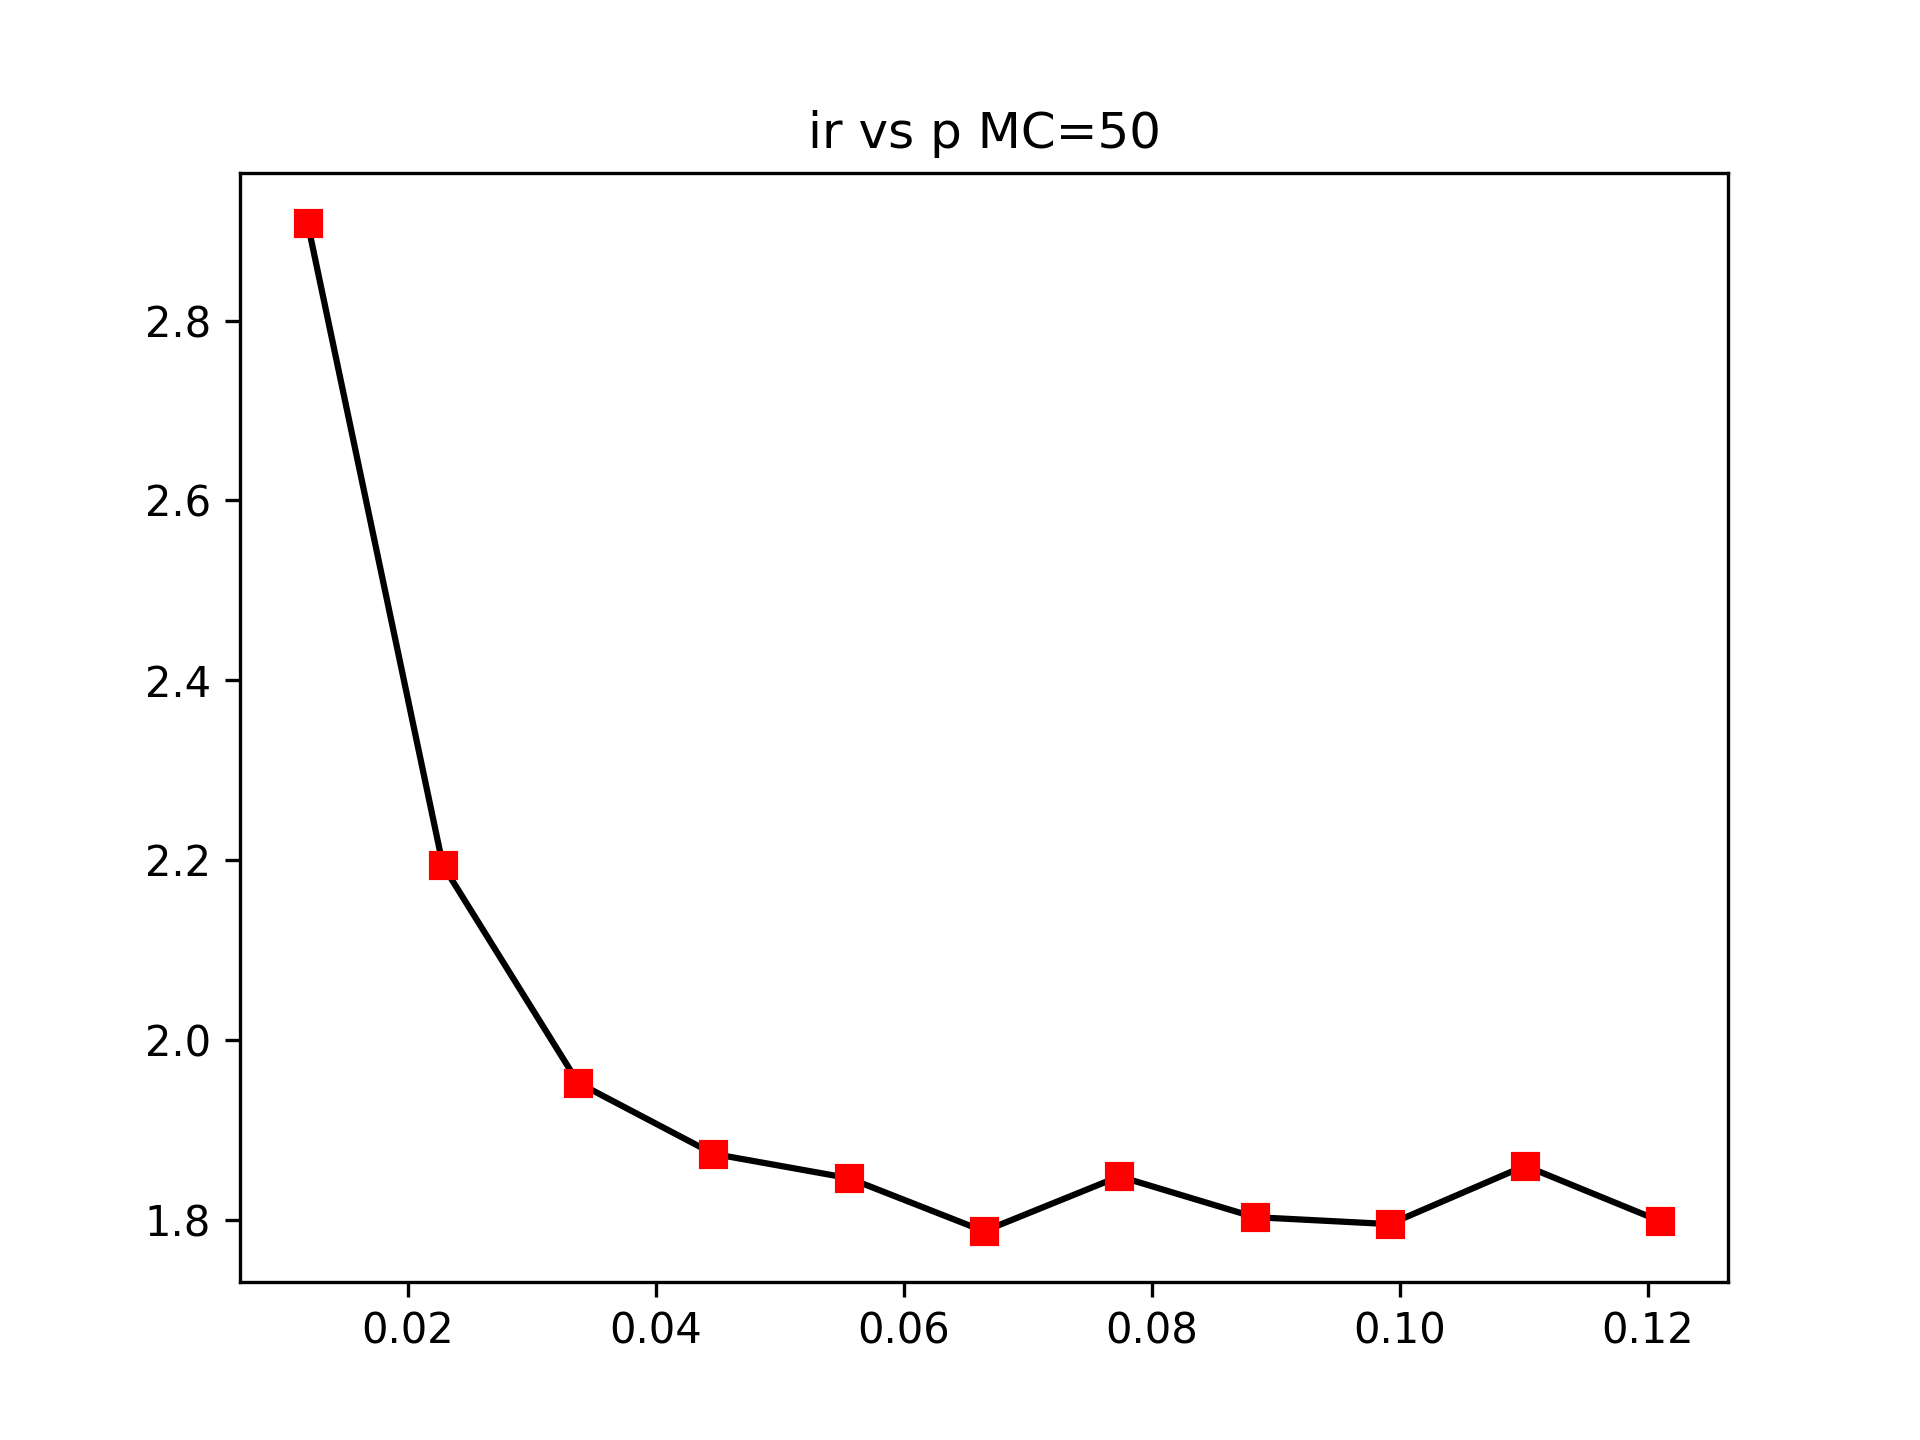
\includegraphics[width=\textwidth, trim=0 0 0 38, clip]{ir.png}
      \end{figure}
    \end{column}
    \begin{column}{0.23\textwidth}
      \centering
      \tiny\renewcommand{\arraystretch}{0.85}\setlength{\tabcolsep}{3pt}
      \begin{tabular}{lr}
        \toprule
        $p$ &  $r^i$ \\
        \midrule
        0.012 & 2.9083 \\
        0.023 & 2.1940 \\
        0.034 & 1.9521 \\
        0.045 & 1.8731 \\
        0.056 & 1.8461 \\
        0.066 & 1.7871 \\
        0.077 & 1.8480 \\
        0.088 & 1.8027 \\
        0.099 & 1.7949 \\
        0.110 & 1.8598 \\
        0.121 & 1.7982 \\
        \bottomrule
      \end{tabular}
    \end{column}
  \end{columns}
\end{frame}

\begin{frame}{Market power $\psi$}
  \tiny Market power $\psi$ decreases monotonically as connectivity $p$ increases. In a denser network, competition among lenders intensifies, eroding the monopolistic markup. This is the mechanism through which connectivity drives interest rates downward.
  \begin{columns}[T]
    \begin{column}{0.75\textwidth}
            \begin{figure}
        \centering
        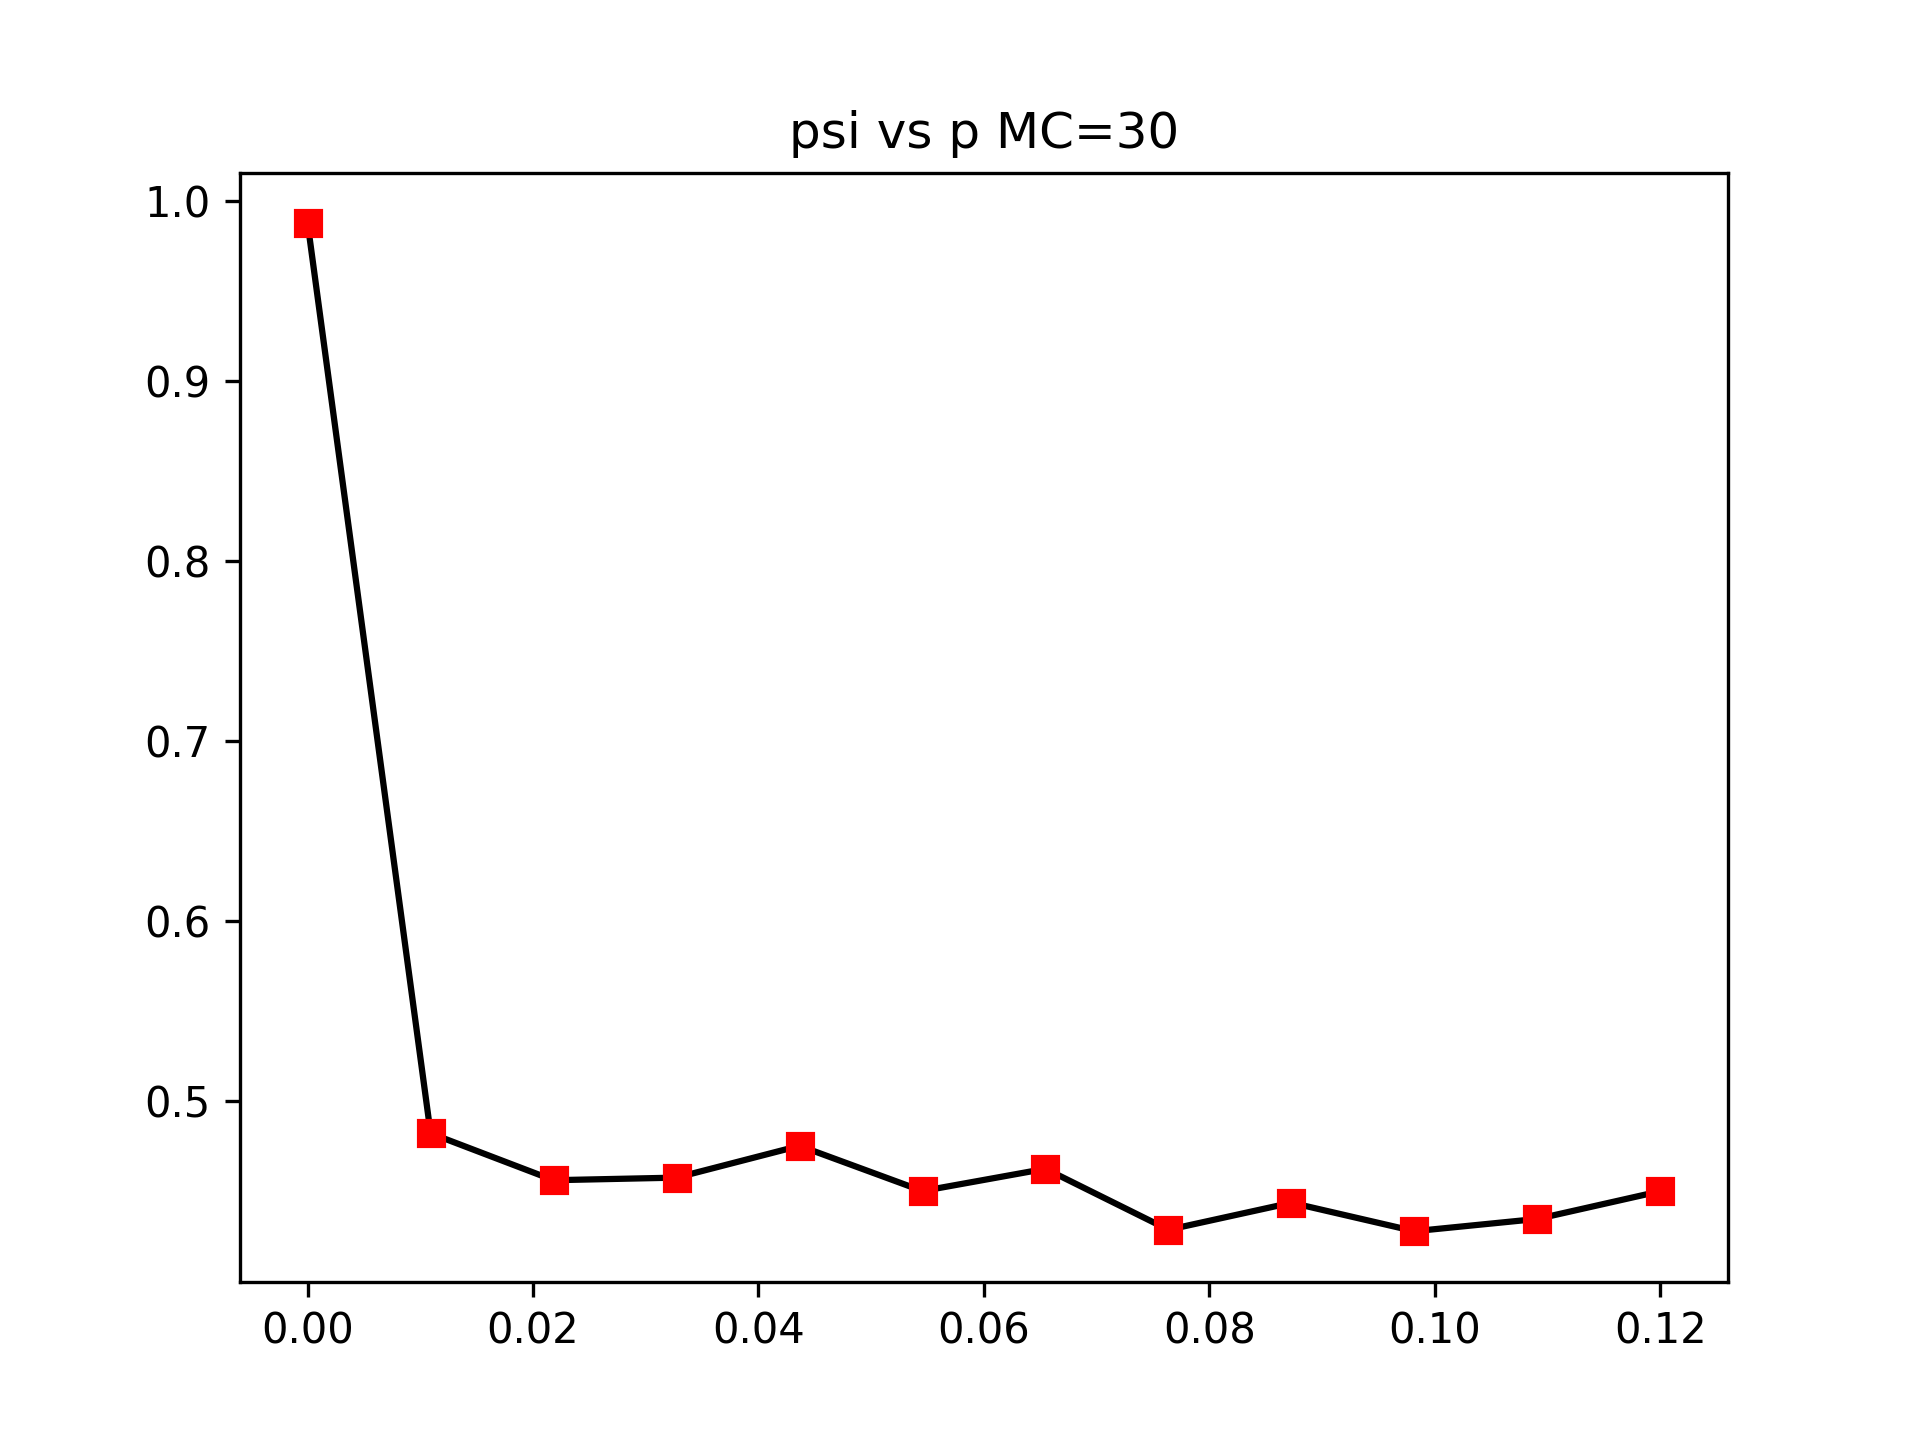
\includegraphics[width=\textwidth, trim=0 0 0 38, clip]{psi.png}
      \end{figure}
    \end{column}
    \begin{column}{0.23\textwidth}
      \centering
      \tiny\renewcommand{\arraystretch}{0.85}\setlength{\tabcolsep}{3pt}
      \begin{tabular}{lr}
        \toprule
        $p$ & $\psi$ \\
        \midrule
        0.012 & 0.4961 \\
        0.023 & 0.4864 \\
        0.034 & 0.4798 \\
        0.045 & 0.4778 \\
        0.056 & 0.4746 \\
        0.066 & 0.4721 \\
        0.077 & 0.4701 \\
        0.088 & 0.4665 \\
        0.099 & 0.4631 \\
        0.110 & 0.4600 \\
        0.121 & 0.4593 \\
        \bottomrule
      \end{tabular}
    \end{column}
  \end{columns}
\end{frame}

\begin{frame}{Probability of bankruptcy $p_b$}
  \tiny As connectivity increases, the probability of borrower bankruptcy rises. Lenders attempt to serve a larger number of clients, and the decline in interest rates reduces the screening incentive, making the system more fragile.
  \begin{columns}[T]
    \begin{column}{0.75\textwidth}
      \begin{figure}
        \centering
        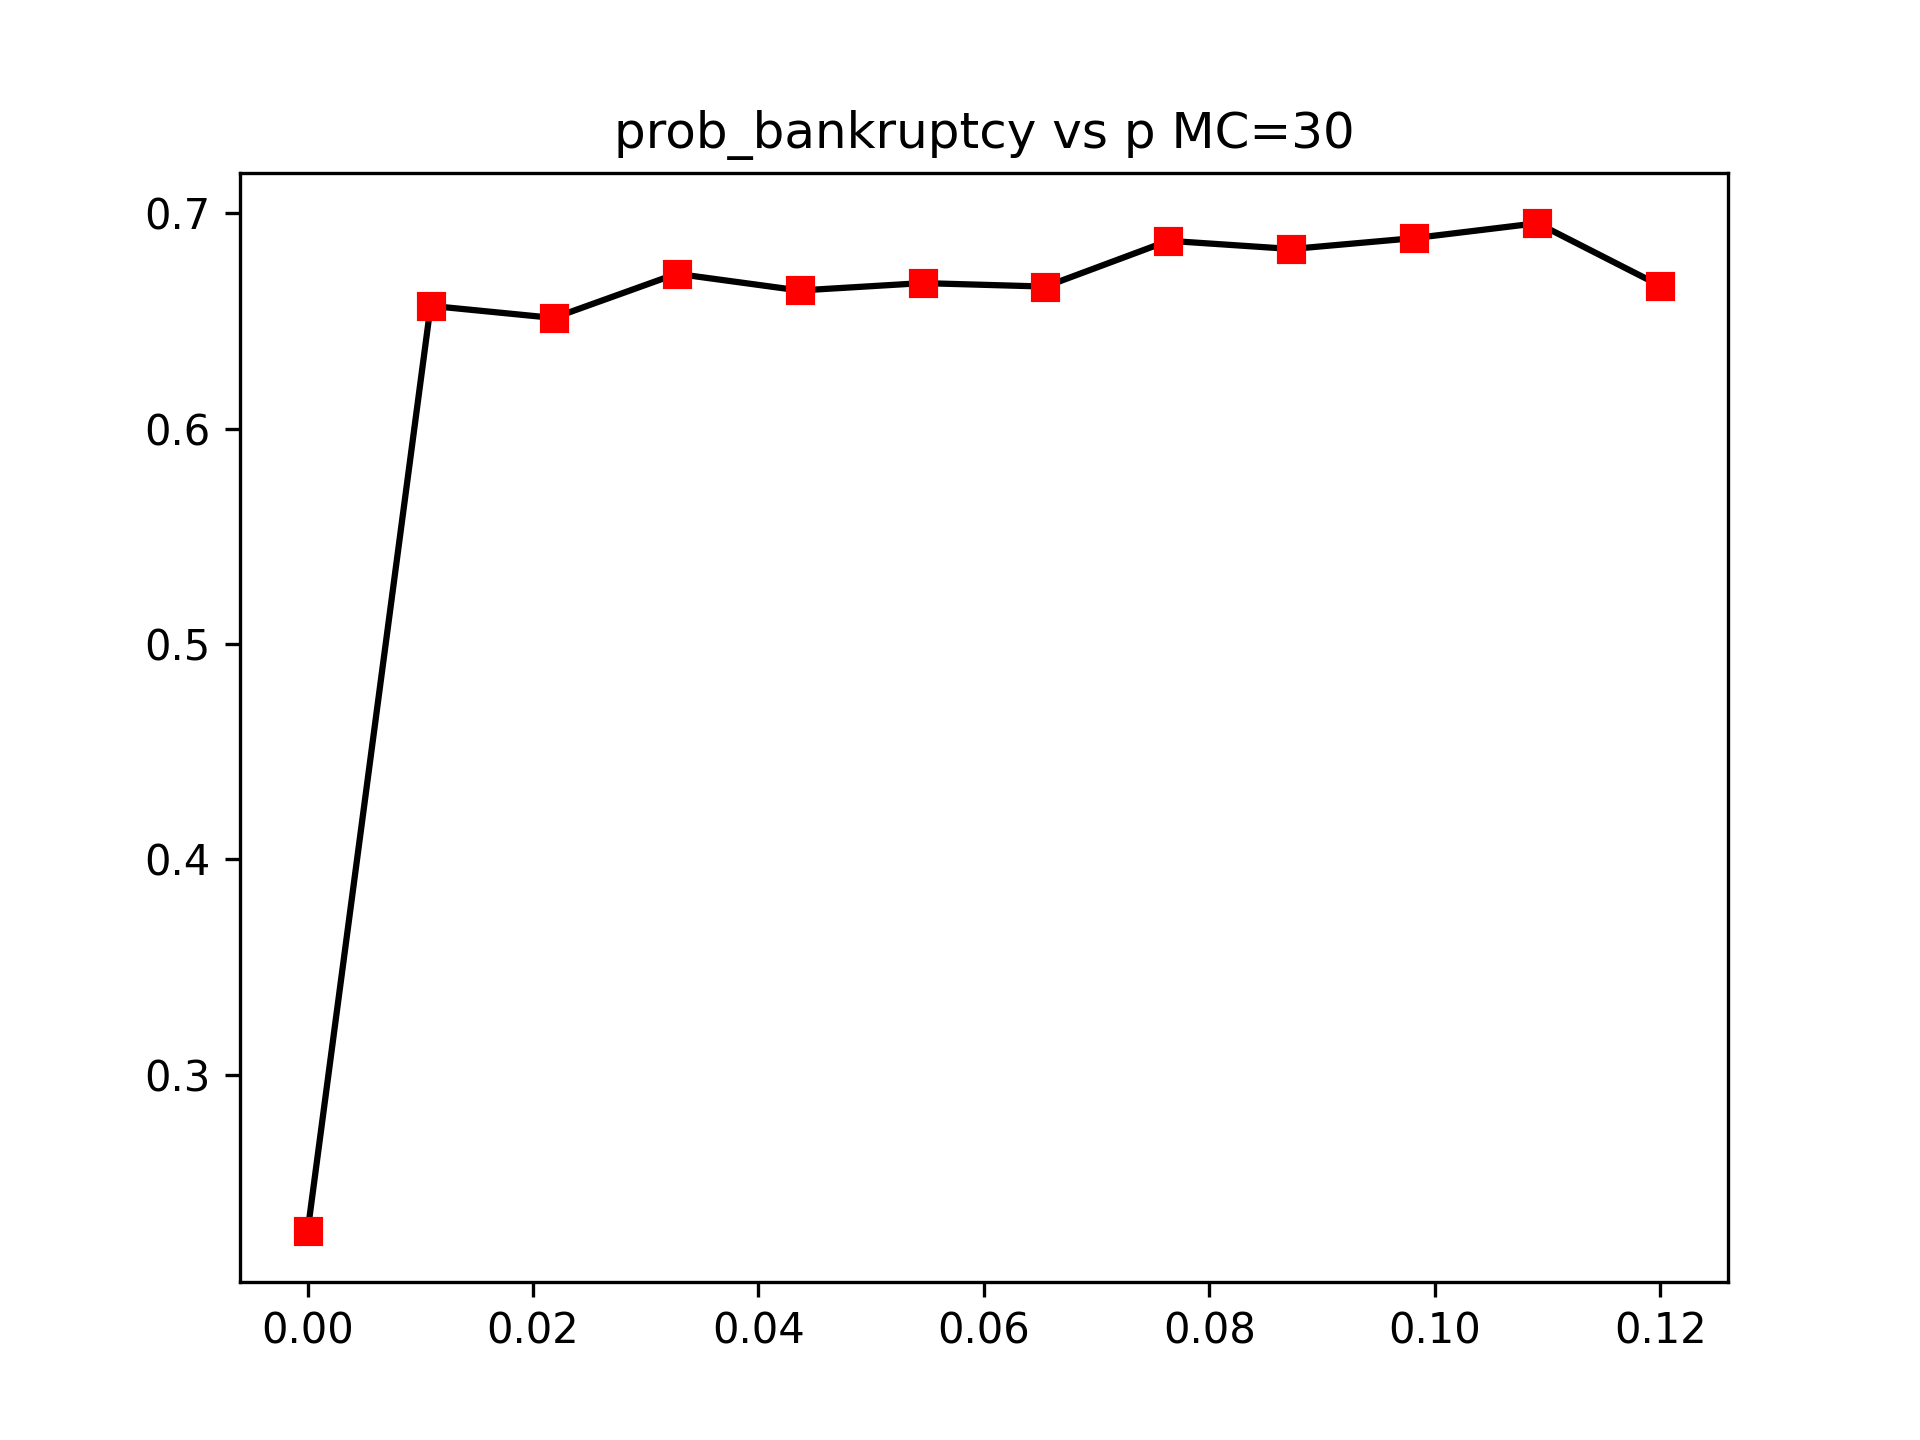
\includegraphics[width=\textwidth, trim=0 0 0 38, clip]{prob_bankruptcy.png}
      \end{figure}
    \end{column}
    \begin{column}{0.23\textwidth}
      \centering
      \tiny\renewcommand{\arraystretch}{0.85}\setlength{\tabcolsep}{3pt}
      \begin{tabular}{lr}
        \toprule
        $p$ & $p_b$\\
        \midrule
        0.012 & 0.6264 \\
        0.023 & 0.6468 \\
        0.034 & 0.6529 \\
        0.045 & 0.6558 \\
        0.056 & 0.6592 \\
        0.066 & 0.6606 \\
        0.077 & 0.6633 \\
        0.088 & 0.6632 \\
        0.099 & 0.6652 \\
        0.110 & 0.6664 \\
        0.121 & 0.6667 \\
        \bottomrule
      \end{tabular}
    \end{column}
  \end{columns}
\end{frame}

\begin{frame}{Bad debt}
  \tiny Bad debt grows with connectivity: more loans are extended as $p$ increases, and a higher volume of lending translates into greater accumulated losses from default. This amplifies the systemic cost of low interest rate environments.
  \begin{columns}[T]
    \begin{column}{0.75\textwidth}
      \begin{figure}
        \centering
        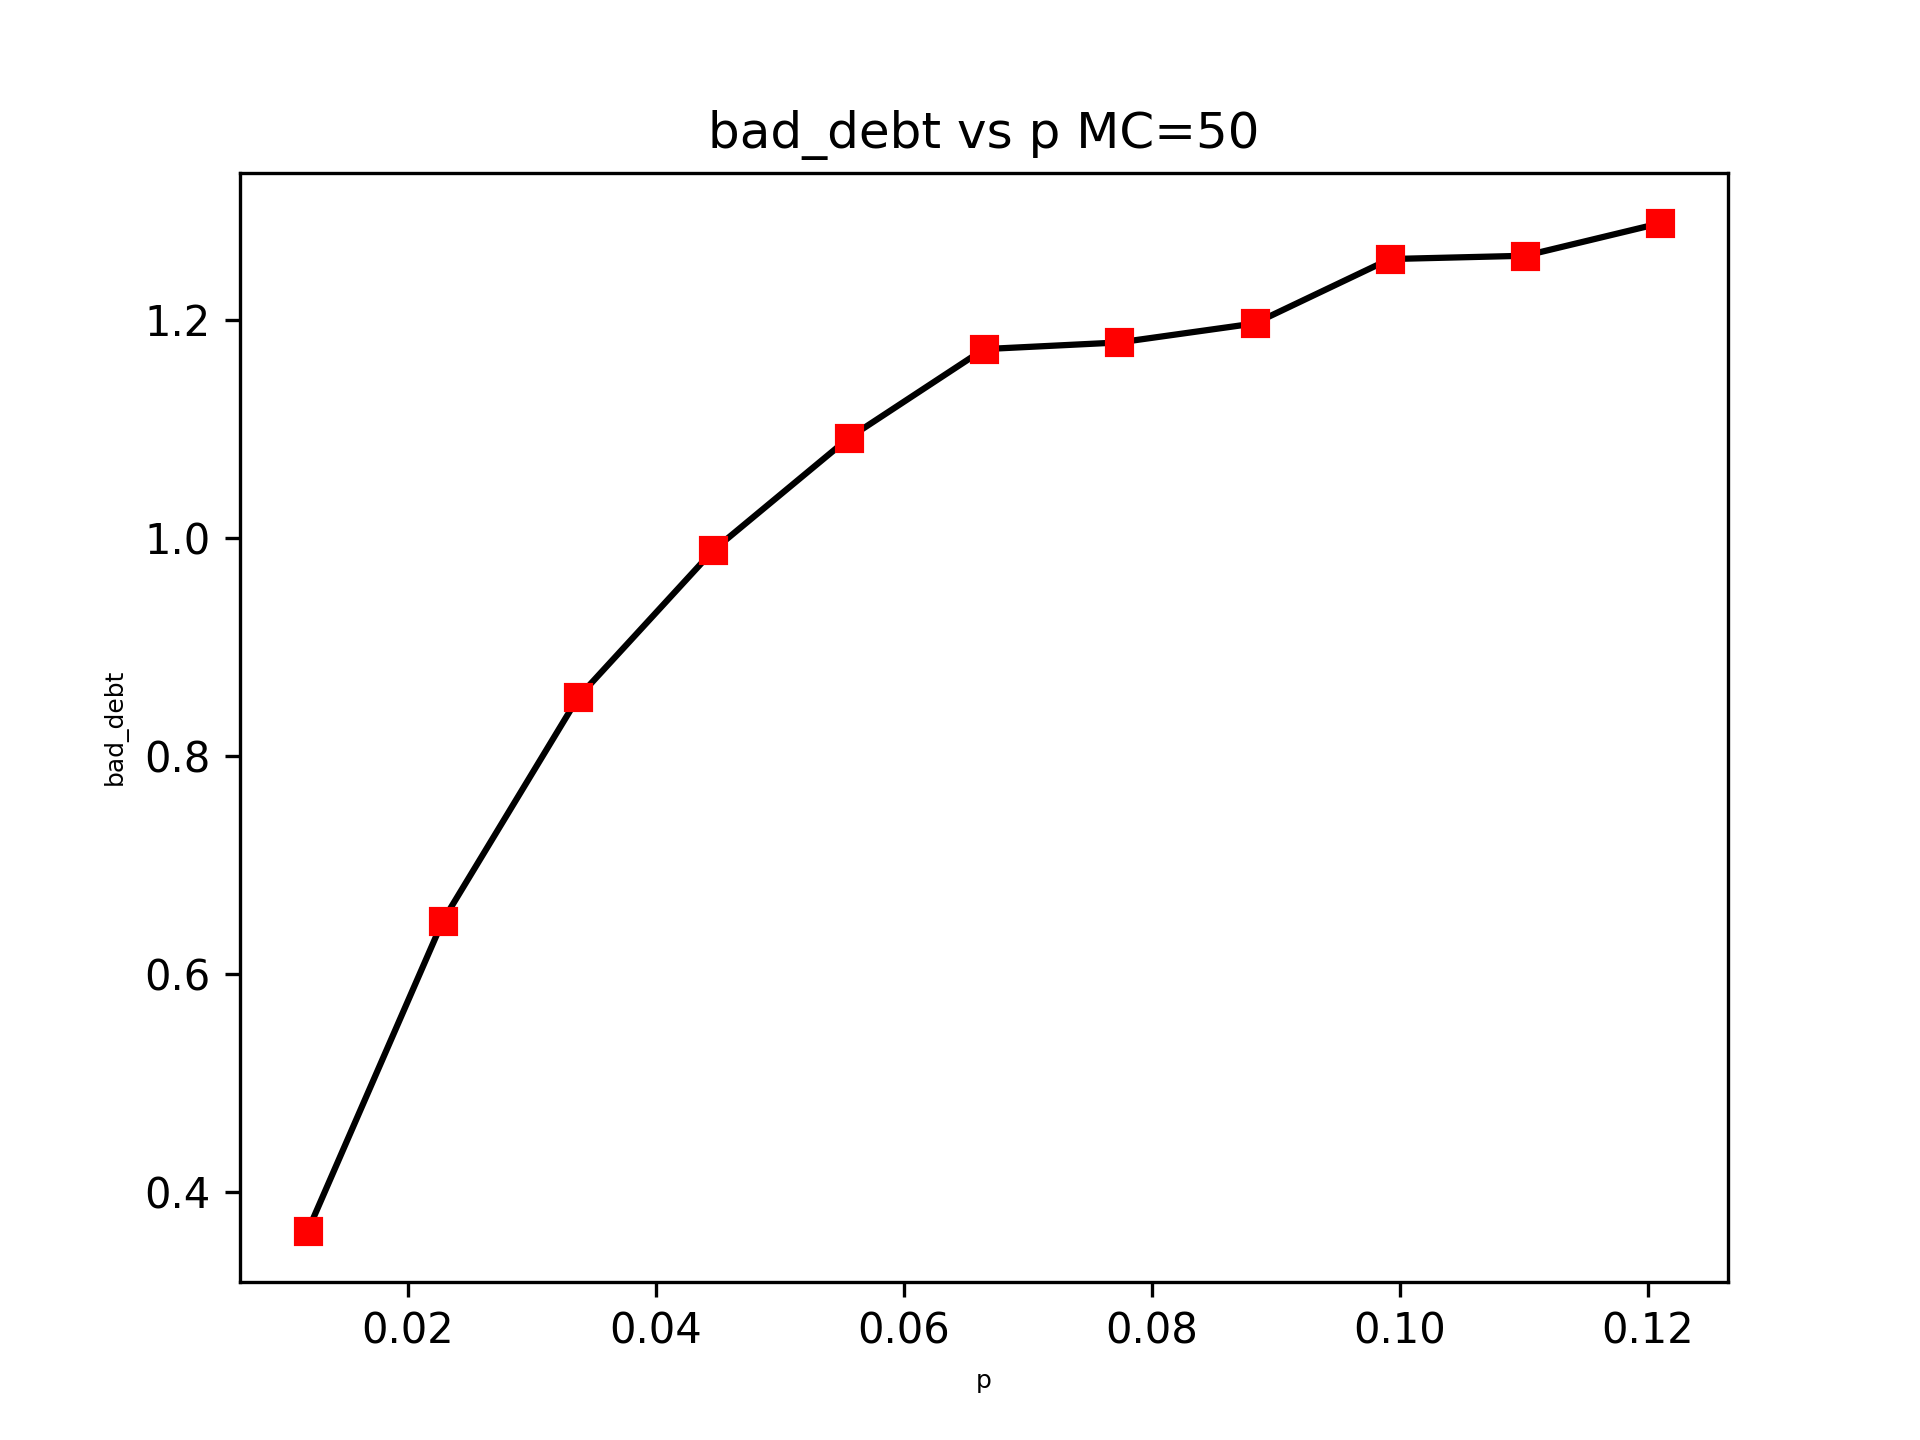
\includegraphics[width=\textwidth, trim=0 0 0 38, clip]{bad_debt.png}
      \end{figure}
    \end{column}
    \begin{column}{0.23\textwidth}
      \centering
      \tiny\renewcommand{\arraystretch}{0.85}\setlength{\tabcolsep}{3pt}
      \begin{tabular}{lr}
        \toprule
        $p$ & $B$ \\
        \midrule
        0.012 & 0.3636 \\
        0.023 & 0.6486 \\
        0.034 & 0.8536 \\
        0.045 & 0.9888 \\
        0.056 & 1.0917 \\
        0.066 & 1.1733 \\
        0.077 & 1.1794 \\
        0.088 & 1.1968 \\
        0.099 & 1.2559 \\
        0.110 & 1.2590 \\
        0.121 & 1.2888 \\
        \bottomrule
      \end{tabular}
    \end{column}
  \end{columns}
\end{frame}


%======================================================================
\section{Conclusions}\label{sec:8}
%======================================================================

\begin{frame}{Key Findings}
  As connectivity $p$ increases:
  \begin{enumerate}
    \item The Giant Component Size increases sharply above the phase transition.
    \item Market power decreases, and the equilibrium interest rate falls.
    \item The probability of borrower bankruptcy rises, as lenders serve a larger number of clients.
    \item Bad debt accumulates, reflecting greater systemic exposure to default.
    \item Taken together, these results show that \textbf{an interest rate that remains too low for too long increases both the incidence of bankruptcies and the spread of contagion}.
  \end{enumerate}
\end{frame}

\begin{frame}{Key Findings}
  \begin{enumerate}
    \item \textbf{Failure composition shifts}: rationing dominates at low $p$; repayment failure dominates at high $p$ as interest rates decline.
    \item The two opposing channels---lower rates from competition, and higher bankruptcy risk from greater connectivity---imply a \textbf{non-trivial trade-off} for regulators.
    \item Excessively low interest rates, while beneficial for borrowers in the short run, can be \textbf{detrimental to the stability of the system} in the long run.
  \end{enumerate}
\end{frame}

\begin{frame}{Policy Implications}
  \begin{itemize}
    \item \textbf{Heterogeneity} is a root cause of systemic instability; the failure of large banks has disproportionate systemic effects.
    \item Interbank lending should ideally be restricted among banks with \textbf{similar liquidity characteristics}.
    \item Reserve requirements dampen cascades but \textbf{constrain growth}.
    %\item Risk diversification across many agents has \textbf{ambiguous} effects on total systemic stability.
    \item \textbf{Monetary policy implications:} an interest rate environment that remains too low for too long can increase connectivity-driven fragility, suggesting that macroprudential policy must account for the endogenous response of network structure.
  \end{itemize}
\end{frame}

\end{document}
